\chapter{Discussion}
Please tell more about conclusion and how to the next work of this study.

\section{Imron Sumadireja / 1164076}
\subsection{Teori}
\begin{enumerate}
\item Jelaskan kenapa file teks harus dilakukan tokenizer. Dilengkapi dengan ilustrasi atau gambar \par
Tokenizer merupakan proses membagi teks yang dapat berupa kalimat, paragraf atau dokumen menjadi kata-kata atau bagian-bagian tertentu dalam kalimat tersebut. Sebagai contoh dari kalimat `Aku mau istirahat dulu ya untuk hari ini', menjadi `Aku', `Mau', `'Istirahat',`Dulu',`Ya',`Untuk',`Hari',`Ini'. Yang menjadi acuan yakni tanda baca dan spasi. Untuk ilustrasinya bisa dilihat pada gambar \ref{toke1}
		\begin{figure}[!htbp]
		\centerline{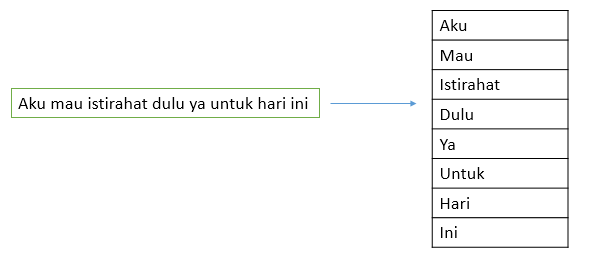
\includegraphics[width=0.5\textwidth]{figures/im/toke1.png}}
		\caption{Ilustrasi Tokenizer.}
		\label{toke1}
		\end{figure}

\end{enumerate}

\section{Yusniar Nur Syarif Sidiq / 1164089}
\subsection{Teori / Yusniar Nur Syarif Sidiq / 1164089}
\begin{enumerate}

\item Jelaskan kenapa file teks harus di lakukan tokenizer. Dilengkapi dengan ilustrasi atau gambar !
	\subitem Sebelumnya kita harus tau terlebih dahulu apa itu Tokenizer, yaitu sebuah proses pembagian terhadap kalimat yang berada dalam dokumen sehingga menjadi sebuah bagian - bagian kata atau bisa kita sebut denga token. Dalam dataset Youtube Tokenizer digunakan untuk melakukan vektorisasi data, sehingga dapat kita simpulkan bahwa data yang telah kita buat dokumen pada chapter 6 yaitu data spam dan bukan spam akan dilakukan vektorisasi dengan menggunakan Tokenizer ini. Ilustrasi sederhana mengenai Tokenizer ini misalkan saya memiliki sebuah kalimat Nama Saya Adalah Yusniar jika gunakan fungsi Tokenizer ini akan dipecah menjadi kata per kata, perhatikan figure \ref{YNC7-1}.

	\begin{figure}[!htbp!]
		\centerline{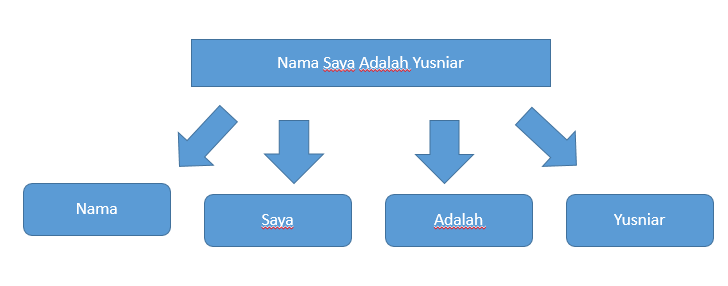
\includegraphics[width=0.5\textwidth]{figures/YN/Chapter7/YNC7-1.png}}
		\caption{Contoh Tokenizer.}
		\label{YNC7-1}
	\end{figure}

\item Jelaskan konsep dasar K Fold Cross Validation pada dataset komentar Youtube !

\item Jelaskan apa maksudnya kode program for train, test in splits. Dilengkapi dengan ilustrasi atau gambar !

\end{enumerate}